\documentclass[8pt,compress]{beamer}
\setbeamertemplate{navigation symbols}{}

\usepackage{graphicx}
\graphicspath{{./FIGURES/}}
\usepackage{color}
\usepackage[utf8x]{inputenc}
% \usepackage{beamerthemetree}
% \usepackage{beamerthemelined}
% \usepackage{beamerthemesplit}
\usepackage{amsmath}
\usepackage{amssymb}
\usepackage{amsthm}
\usepackage{draftcopy}
\usepackage{fontenc}
\usepackage{graphicx}
\usepackage{pgf}
\usepackage{times}
\usepackage{tikz}
\usepackage[T1]{fontenc}
\usepackage{verbatim}

% \usetheme{Warsaw}
% \usetheme{Rochester}
% \usetheme{bars}
% \usetheme{Bergen}
% \usetheme{Boadilla}
% \usetheme{Boxes}
% \usetheme{classic}
% \usetheme{Madrid}
% \usetheme{Pittsburgh}
% \usetheme{Antibes}
% \usetheme{Montpellier}
% \usetheme{Berkeley}
% \usetheme{PaloAlto}
% \usetheme{Goettingen}
% \usetheme{Marburg}
% \usetheme{Hannover}
% \usetheme{JuanLesPins}
% \usetheme{Berlin}
% \usetheme{Ilmenau}
% \usetheme{Dresden}
% \usetheme{Luebeck}
% \usetheme{Darmstadt}
% \usetheme{Frankfurt}
% \usetheme{Singapore}
% \usetheme{Szeged}
\usetheme{Copenhagen}
% \usetheme{lined}
% \usetheme{Malmoe}
% \usetheme{Tree}
% \usetheme{shadow}
% \usetheme{sidebar}
% \usetheme{split}
% \usetheme{default}
\setbeamercovered{transparent}

%%%%%%%%%% Choose color scheme%%%%%%%%
\usecolortheme{default}
% \usecolortheme{sidebartab}
% \usecolortheme{albatross}
% \usecolortheme{beetle}
% \usecolortheme{crane}
% \usecolortheme{dolphin}
% \usecolortheme{dove}
% \usecolortheme{fly}
% \usecolortheme{seagull}
% \usecolortheme{lily}
% \usecolortheme{orchid}
% \usecolortheme{seahorse}
% \usecolortheme{rose}
% \usecolortheme{whale}
% \usecolortheme{structure}
%%%%%%%%%%%%%%%%%%%%%%%%%%%%%%%%%%%

% \useoutertheme{shadow}
\useoutertheme{infolines}
% \useoutertheme{split}

% * Redistribute the spaces in the foot line
% * Set the author without institution
\defbeamertemplate*{footline}{infolines}
{
    \leavevmode%
    \hbox{%
    \begin{beamercolorbox}[wd=.25\paperwidth,ht=2.25ex,dp=1ex,center]{author in head/foot}%
		\usebeamerfont{author in head/foot}Jose Luis Cercos-Pita
    \end{beamercolorbox}%
    \begin{beamercolorbox}[wd=.5\paperwidth,ht=2.25ex,dp=1ex,center]{title in head/foot}%
        \usebeamerfont{title in head/foot}\insertshorttitle
    \end{beamercolorbox}%
    \begin{beamercolorbox}[wd=.25\paperwidth,ht=2.25ex,dp=1ex,right]{date in head/foot}%
        \usebeamerfont{date in head/foot}\insertshortdate{}\hspace*{2em}
        \insertframenumber{} / \inserttotalframenumber\hspace*{2ex}
    \end{beamercolorbox}}%
    \vskip0pt%
}

\newcommand{\CC}{C\nolinebreak\hspace{-.30em}\raisebox{.2ex}{ +}\nolinebreak\hspace{-.10em}\raisebox{.2ex}{+}}

% \hypersetup{pdfpagemode=FullScreen}

\usepackage{tikz}
\usetikzlibrary{calc,shapes}
\tikzstyle{yellowbox}=[rectangle,draw=black,fill=yellow,
                       font=\scriptsize\sffamily\bfseries,inner sep=6pt]
\tikzstyle{greybox}=[rectangle,draw=black,fill=gray,
                     font=\scriptsize\sffamily\bfseries,inner sep=2pt]
\tikzstyle{whitebox}=[rectangle,draw=black,fill=white,
                      font=\scriptsize\sffamily\bfseries,inner sep=2pt]
\tikzstyle{arr}=[-latex,black,line width=1pt]
\newcommand\nodelabel[3][30em]{\parbox{#1}{\centering #2 \\ #3 }}
\newcommand\nodelabell[3][21em]{\parbox{#1}{\centering #2 \\ #3 }}
\newcommand\vertspacing{-1.0}

\AtBeginSection[]
{
  \begin{frame}
  \frametitle{Contents}
  \tableofcontents[currentsection]
  \end{frame}
}

\begin{document}

\title{SonSilentSea, creación de juegos en Blender con Python}  
\author{Jose Luis Cercos-Pita}
\date{\today} 

\begin{frame}
\titlepage
\end{frame}

\begin{frame} \frametitle{Tabla de contenidos}
\tableofcontents
\end{frame} 

\section{Introducción} 

\subsection{¿Quién soy yo?}
\begin{frame}{¿Quién soy yo?}
	\begin{itemize}
		\item Ingeniero Naval y Oceánico
		\item Doctorando del programa de ingeniería aeroespacial
		\item Investigador en el canal de ensayos de la ETSIN
		\item Especializado en mecánica de fluidos computacional
		\item Desarrollador de software libre
		\begin{itemize}
			\item FreeCAD
			\item ocland
			\item SonSilentSea
			\item ...
		\end{itemize}	
	\end{itemize}
\end{frame}

\subsection{¿Qué es SonSilentSea?}
\begin{frame}{¿Qué es SonSilentSea?}
	\begin{center}
	\href{https://github.com/sanguinariojoe/sonsilentsea}{https://github.com/sanguinariojoe/sonsilentsea}
	\end{center}
	\begin{itemize}
		\item Juego de simulación naval
		\item Dedicado a Sonsoles Jiménez Caballero
		\item Software libre
		\item Desarrollado durante 3 años con \CC $\,$ y OGRE
		\item Ahora se desarrolla en Blender con Python
	\end{itemize}
	\begin{figure}
		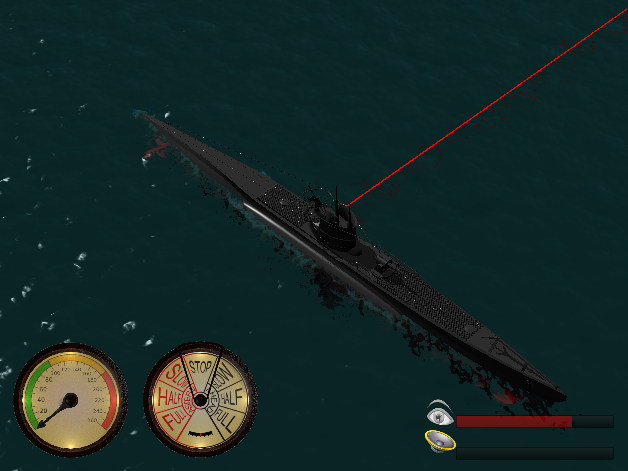
\includegraphics[scale=0.3]{screenshot0} 
	\end{figure}
\end{frame}

\subsection{¿Qué pretendo contar?}
\begin{frame}{¿Qué pretendo contar?}
	\begin{itemize}
		\item OGRE vs. Blender
		\item \textbf{\CC $\,$ vs. Python}
	\end{itemize}
	%
	\pause
	%
	O más concretamente...
	%
	\begin{itemize}
		\item Diferencias debidas a la familiaridad con el diseño,
		el lenguaje y el entorno
		% 1.- Familiaridad con el lenguaje y el entorno
		% 2.- Claridad en el diseño
		\item Diferencias debidas a una mejor integración
		% 1.- Exportacion de modelos
		%  1.b.- Zonas de suavizado
		%  1.c.- Materiales
		%  1.d.- Sistemas de referencia
		%  1.e.- Ligaduras
		% 2.- Particulas
		% 3.- Posibilidades para extender
		% 4.- Adaptacion a las necesidades
		\item Diferencias debidas a tener un framework
		% 1.- Fisicas
		% 2.- Entradas y salidas
		% 3.- Operadores logicos
		% 4.- Limitaciones
		%  4.a.- Limitacion de masa
		%  4.b.- Orden de renderizado
		\item Diferencias debidas a los estándares (ligado con la integración)
		% 1.- Modularizacion
		% 2.- CEGUI vs. bgui
		% 3.- Fragmentacion
		% 4.- Portabilidad
		\item \textbf{Diferencias debidas al lenguaje (\CC $\,$ vs. Python)}
		% 1.- Lineas de codigo
		% 2.- Errores y debugado
		% 3.- Campañas (directamente en Python frente al parser XML)
	\end{itemize}

	\vspace{0.3cm}

	\begin{center}
		Tratamos de estimar que parte se límita al cambio de lenguaje,
		pero es difícil de medir: tiempo, esfuerzo, cantidad de información...
		
		"3 años en \CC $\,$ $\rightarrow$ 2 meses en Python"
	\end{center}
	%
\end{frame}

\begin{frame}{Precedentes}
Usando algunos ejemplos de algoritmos de ordenación...

\vspace{0.5cm}
\begin{columns}
  \begin{column}{0.5\textwidth}
    \textbf{\underline{Python}}
    \begin{itemize}
        \item Bubble sort: 24 líneas
        \item Bitonic sort: 23 líneas
        \item Counting sort: 11 líneas
        \item Insertion sort: 8 líneas
        \item Merge sort: 24 líneas
        \item Heap sort: 35 líneas
        \item Radix sort: 38 líneas
    \end{itemize}
  \end{column}

  \begin{column}{0.5\textwidth}
    \textbf{\underline{\CC}}
    \begin{itemize}
        \item Bubble sort: 33 líneas (x1.4)
        \item Bitonic sort: 131 líneas (x5.7)
        \item Counting sort: 49 líneas (x4.5)
        \item Insertion sort: 9 líneas (x1.1)
        \item Merge sort: 58 líneas (x2.4)
        \item Heap sort: 53 líneas (x1.5)
        \item Radix sort: 90 líneas (x2.4)
    \end{itemize}
  \end{column}
\end{columns}

\vspace{0.5cm}
Con ésta pequeña muestra crear un algoritmo en C++ parece requerir
$2.7 \pm 1.6$ veces más líneas de código

\end{frame}

\begin{frame}{Diferencias en cuanto a características}
\begin{columns}
  \begin{column}{0.5\textwidth}
    \textbf{\underline{Blender}}
    \begin{itemize}
        \item 20 FPS en el portátil
        \item Cámara "isométrica"
        \item Sólo visión desde fuera del agua
        \item Geometría del mar simplificada por un plano
        \item Física más realista
        \item No existe necesidad de preocuparse por la atmósfera
    \end{itemize}
	\begin{figure}
		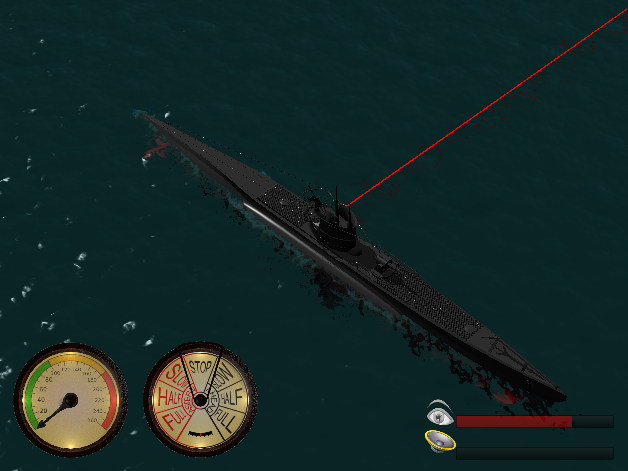
\includegraphics[scale=0.22]{screenshot0} 
	\end{figure}    
  \end{column}

  \begin{column}{0.5\textwidth}
    \textbf{\underline{OGRE}}
    \begin{itemize}
        \item Inmanejable en el portátil
        \item Cámara libre
        \item Completo entorno submarino (Hydrax)
        \item Compleja geometría del mar
        \item Física pobre
        \item Atmósfera realista (SkyX)
    \end{itemize}
	\begin{figure}
		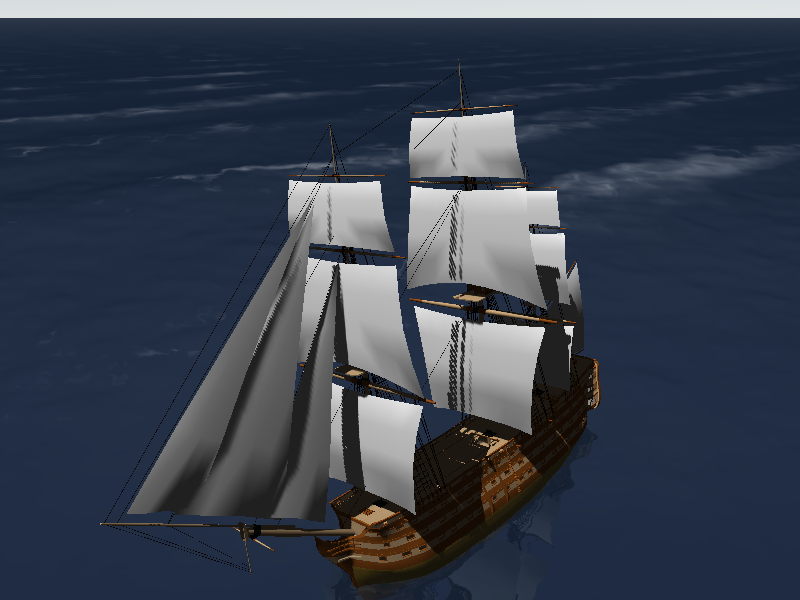
\includegraphics[scale=0.18]{old_screenshot_6} 
	\end{figure}
  \end{column}
\end{columns}
\end{frame}


\section{Líneas de código} 

\subsection{Estructura general} 
\begin{frame}{Estructura general}
\begin{columns}
  \begin{column}{0.5\textwidth}
    \textbf{\underline{Blender}}
    
    7975 líneas de código
    
    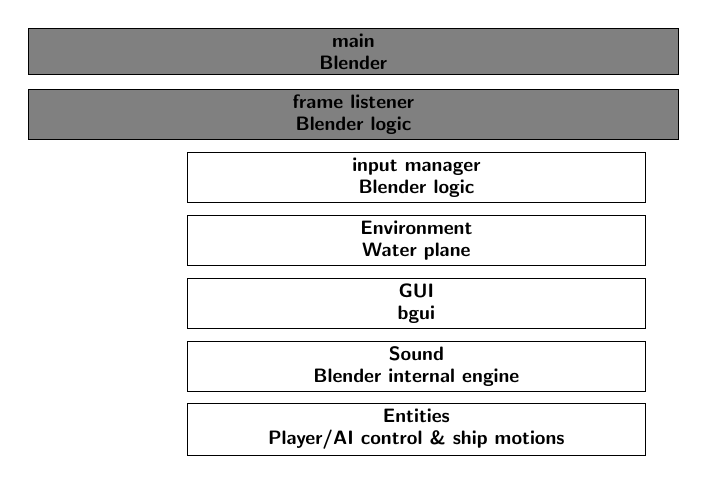
\begin{tikzpicture}[scale=0.8]
    	\node [greybox] (main) at ($(-5,\vertspacing*1)$) {
    		\nodelabel{main}{\textit{Blender}}
    	};
    	\node [greybox] (frame listener) at ($(-5,\vertspacing*2)$) {
    		\nodelabel{frame listener}{\textit{Blender logic}}
    	};
    	\node [whitebox] (input manager) at ($(-4,\vertspacing*3)$) {
    		\nodelabell{input manager}{\textit{Blender logic}}
    	};
    	\node [whitebox] (Environment) at ($(-4,\vertspacing*4)$) {
    		\nodelabell{Environment}{\textit{Water plane}}
    	};
    	\node [whitebox] (GUI) at ($(-4,\vertspacing*5)$) {
    		\nodelabell{GUI}{\textit{bgui}}
    	};
    	\node [whitebox] (Sound) at ($(-4,\vertspacing*6)$) {
    		\nodelabell{Sound}{\textit{Blender internal engine}}
    	};
    	\node [whitebox] (Entities) at ($(-4,\vertspacing*7)$) {
    		\nodelabell{Entities}{\textit{Player/AI control \& ship motions}}
    	};
    \end{tikzpicture}
  \end{column}

  \begin{column}{0.5\textwidth}
    \textbf{\underline{OGRE}}

	39211 líneas de código (\textcolor{red}{-1054} líneas)

    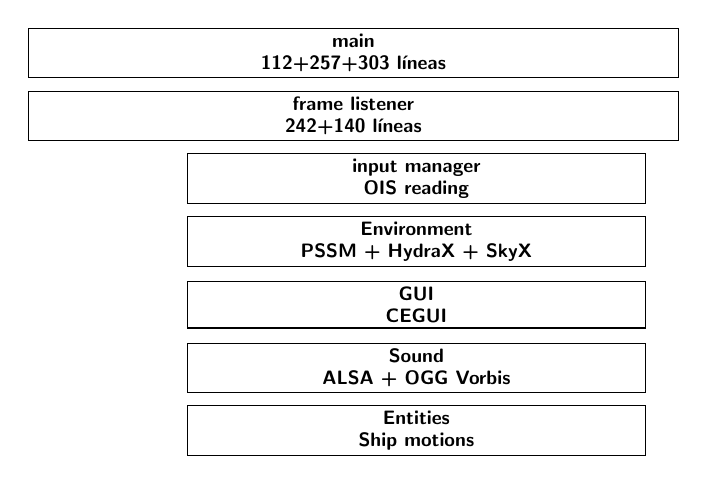
\begin{tikzpicture}[scale=0.8]
    	\node [whitebox] (main) at ($(-5,\vertspacing*1)$) {
    		\nodelabel{main}{\textit{112+257+303 líneas}}
    	};
    	\node [whitebox] (frame listener) at ($(-5,\vertspacing*2)$) {
    		\nodelabel{frame listener}{\textit{242+140 líneas}}
    	};
    	\node [whitebox] (input manager) at ($(-4,\vertspacing*3)$) {
    		\nodelabell{input manager}{\textit{OIS reading}}
    	};
    	\node [whitebox] (Environment) at ($(-4,\vertspacing*4)$) {
    		\nodelabell{Environment}{\textit{PSSM + HydraX + SkyX}}
    	};
    	\node [whitebox] (GUI) at ($(-4,\vertspacing*5)$) {
    		\nodelabell{GUI}{\textit{CEGUI}}
    	};
    	\node [whitebox] (Sound) at ($(-4,\vertspacing*6)$) {
    		\nodelabell{Sound}{\textit{ALSA + OGG Vorbis}}
    	};
    	\node [whitebox] (Entities) at ($(-4,\vertspacing*7)$) {
    		\nodelabell{Entities}{\textit{Ship motions}}
    	};
    \end{tikzpicture}
  \end{column}
\end{columns}
\end{frame}

\subsection{Componentes} 
\begin{frame}{Input manager}
\begin{columns}
  \begin{column}{0.5\textwidth}
    \textbf{\underline{Blender}} (0 líneas)
    
	\begin{figure}
		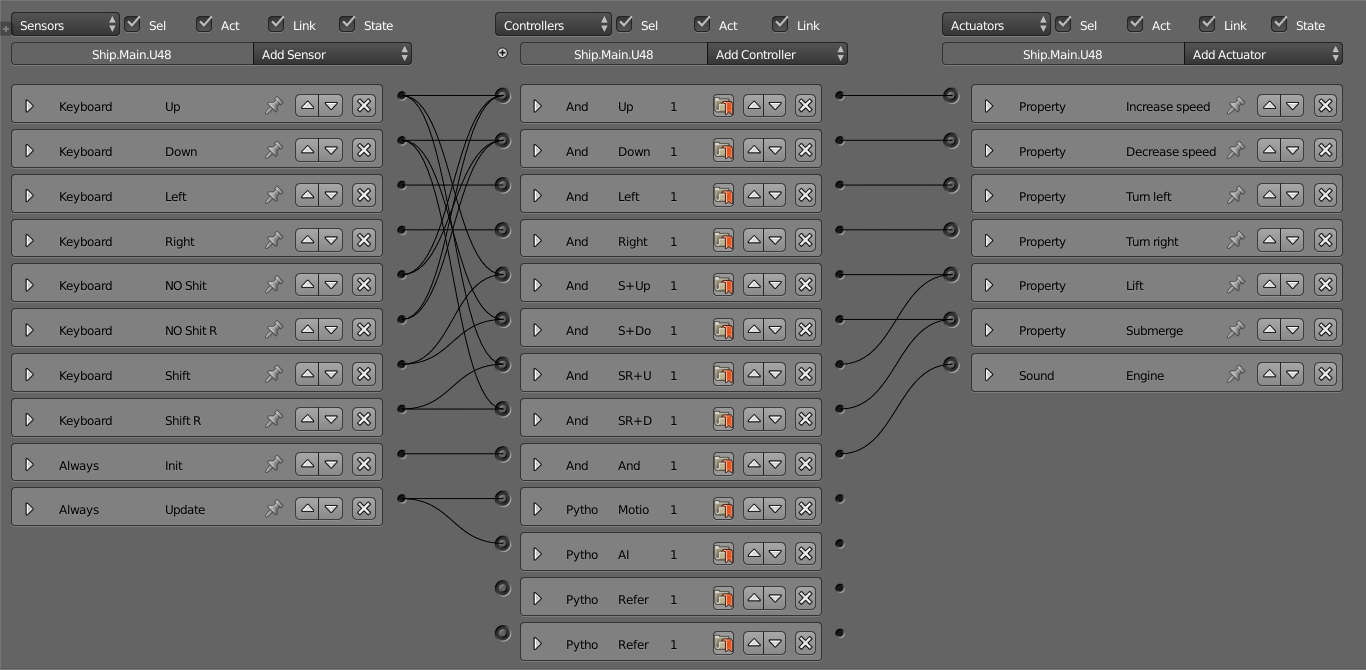
\includegraphics[scale=0.12]{blender_logic} 
	\end{figure}
  \end{column}

  \begin{column}{0.5\textwidth}
    \textbf{\underline{OGRE}} (\textcolor{red}{-1054-379} líneas)
    
    \vspace{0.4cm}
    Analizar las entradas por teclado y ratón en \CC $\,$ requiere generar una
    clase específica para ello haciendo uso de OIS (el estándar en OGRE hasta
    la versión 1.8).
    
    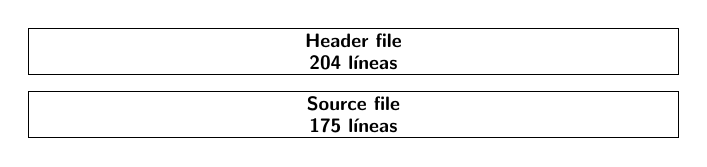
\begin{tikzpicture}[scale=0.8]
    	\node [whitebox] (Header file) at ($(-5,\vertspacing*1)$) {
    		\nodelabel{Header file}{\textit{204 líneas}}
    	};
    	\node [whitebox] (Source file) at ($(-5,\vertspacing*2)$) {
    		\nodelabel{Source file}{\textit{175 líneas}}
    	};
    \end{tikzpicture}    
  \end{column}
\end{columns}
\end{frame}

\begin{frame}{Input manager}
\begin{columns}
  \begin{column}{0.5\textwidth}
    \textbf{\underline{Blender}} (\textcolor{red}{-98} líneas)
    
    \vspace{0.5cm}
    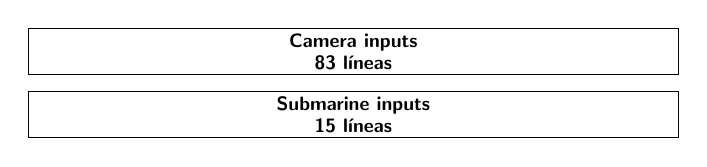
\begin{tikzpicture}[scale=0.8]
    	\node [whitebox] (Camera inputs) at ($(-5,\vertspacing*1)$) {
    		\nodelabel{Camera inputs}{\textit{83 líneas}}
    	};
    	\node [whitebox] (Submarine inputs) at ($(-5,\vertspacing*2)$) {
    		\nodelabel{Submarine inputs}{\textit{15 líneas}}
    	};
    \end{tikzpicture}	
  \end{column}

  \begin{column}{0.5\textwidth}
    \textbf{\underline{OGRE}} (\textcolor{red}{-1054-379} líneas)
    
    \vspace{1.5cm}
    Sin implementar en OGRE
  \end{column}
\end{columns}
\end{frame}

\begin{frame}{Environment (Parallel-Split Shadow Maps)}
%
\begin{itemize}
	\item Crucial para obtener sombras de calidad.
	\item Crítico en función de la distancia mínima de corte:
	\[
	\left( \begin{matrix} x_v \\ y_v \\ z_v \\ w_v \end{matrix} \right)	
	=
	\left( \begin{matrix} 
		\frac{n}{r} & 0           & 0                & 0                  \\
		0           & \frac{n}{h} & 0                & 0                  \\
		0           & 0           & -\frac{f+n}{f-n} & -\frac{2 f n}{f-n} \\
		0           & 0           & -1               & 0                  \\
	\end{matrix} \right)	
	\left( \begin{matrix} x \\ y \\ z \\ w \end{matrix} \right)	
	,
	\]
	Resultando la profundidad del punto en pantalla como:
	\[ z_s = \frac{z_v}{w_v} = 2 \frac{f n}{f - n} \frac{w}{z} + \frac{f + n}{f - n}
	= \mathcal{O}\left( \frac{1}{z} \right) \]
\end{itemize}
\pause
\hrule
\vspace{0.2cm}
%
\begin{columns}
  \begin{column}{0.5\textwidth}
    \textbf{\underline{Blender}} (\textcolor{red}{-98} líneas)
    
    \vspace{1.2cm}
    Implementado internamente en el motor de Blender.
  \end{column}

  \begin{column}{0.5\textwidth}
    \textbf{\underline{OGRE}} (\textcolor{red}{-1054-379-159} líneas)
        
    \vspace{0.5cm}
    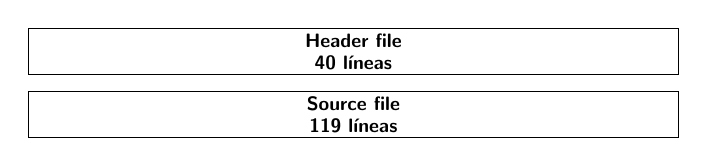
\begin{tikzpicture}[scale=0.8]
    	\node [whitebox] (Header file) at ($(-5,\vertspacing*1)$) {
    		\nodelabel{Header file}{\textit{40 líneas}}
    	};
    	\node [whitebox] (Source file) at ($(-5,\vertspacing*2)$) {
    		\nodelabel{Source file}{\textit{119 líneas}}
    	};
    \end{tikzpicture}    
  \end{column}
\end{columns}
\end{frame}

\begin{frame}{Environment (Atmósfera)}
\begin{columns}
  \begin{column}{0.5\textwidth}
    \textbf{\underline{Blender}} (\textcolor{red}{-98} líneas)
    
    \vspace{0.4cm}
    La cámara no permite apreciar la atmósfera, y por tanto no ha sido implementada.
  \end{column}

  \begin{column}{0.5\textwidth}
    \textbf{\underline{OGRE}} (\textcolor{red}{-1054-379-159-11877} líneas)
    
    \vspace{0.4cm}
    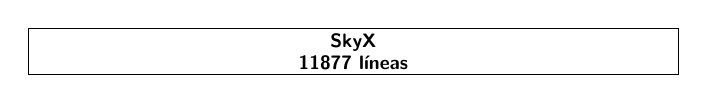
\begin{tikzpicture}[scale=0.8]
    	\node [whitebox] (SkyX) at ($(-5,\vertspacing*1)$) {
    		\nodelabel{SkyX}{\textit{11877 líneas}}
    	};
    \end{tikzpicture}    
  \end{column}
\end{columns}
\begin{figure}
	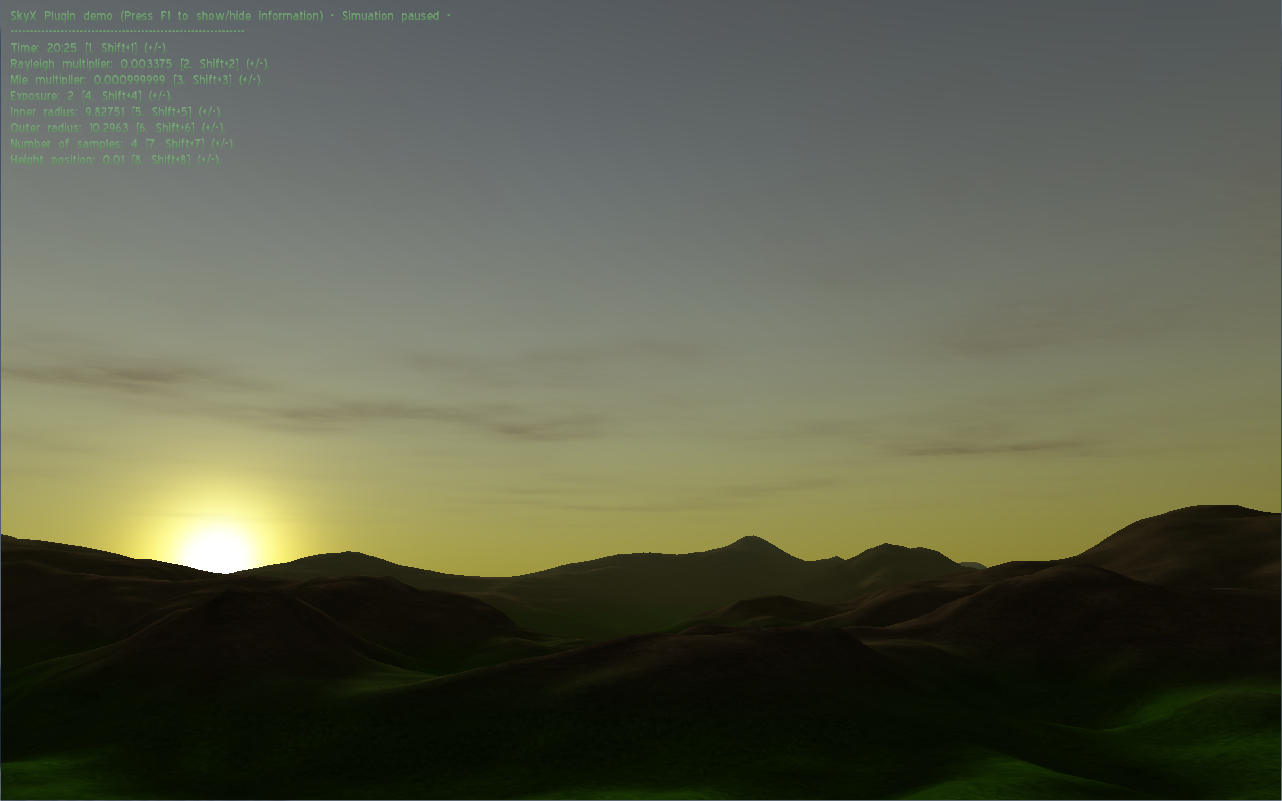
\includegraphics[scale=0.1]{skyx_sky} 
	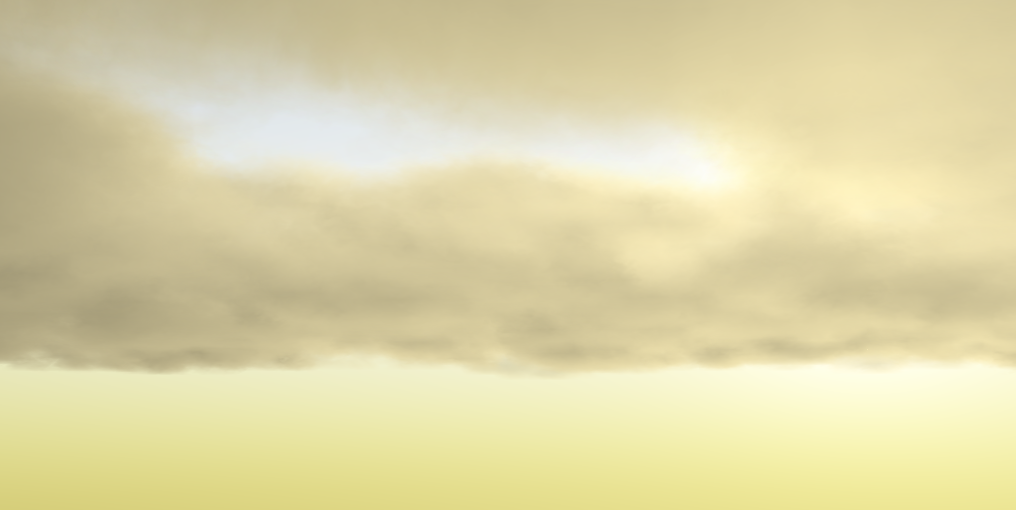
\includegraphics[scale=0.2095]{skyx_clouds} 
\end{figure}
\end{frame}

\begin{frame}{Environment (Océano)}
\begin{columns}
  \begin{column}{0.5\textwidth}
    \textbf{\underline{Blender}} (\textcolor{red}{-98-38} líneas)
    
    \vspace{0.4cm}
    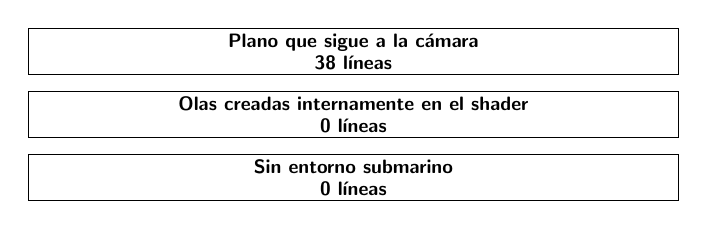
\begin{tikzpicture}[scale=0.8]
    	\node [whitebox] (Plano) at ($(-5,\vertspacing*1)$) {
    		\nodelabel{Plano que sigue a la cámara}{\textit{38 líneas}}
    	};
    	\node [whitebox] (Olas) at ($(-5,\vertspacing*2)$) {
    		\nodelabel{Olas creadas internamente en el shader}{\textit{0 líneas}}
    	};
    	\node [whitebox] (Submarino) at ($(-5,\vertspacing*3)$) {
    		\nodelabel{Sin entorno submarino}{\textit{0 líneas}}
    	};
    \end{tikzpicture}
  \end{column}

  \begin{column}{0.5\textwidth}
    \textbf{\underline{OGRE}} (\textcolor{red}{-1054-379-159-11877-8220} líneas)
    
    \vspace{0.4cm}
    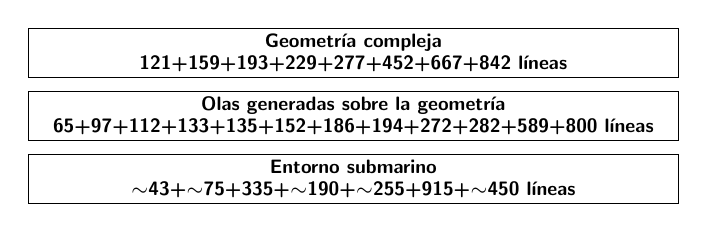
\begin{tikzpicture}[scale=0.8]
    	\node [whitebox] (Geometría compleja) at ($(-5,\vertspacing*1)$) {
    		\nodelabel{Geometría compleja}{\textit{121+159+193+229+277+452+667+842 líneas}}
    	};
    	\node [whitebox] (Olas) at ($(-5,\vertspacing*2)$) {
    		\nodelabel{Olas generadas sobre la geometría}{\textit{65+97+112+133+135+152+186+194+272+282+589+800 líneas}}
    	};
    	\node [whitebox] (Submarino) at ($(-5,\vertspacing*3)$) {
    		\nodelabel{Entorno submarino}{\textit{$\sim$43+$\sim$75+335+$\sim$190+$\sim$255+915+$\sim$450 líneas}}
    	};
    \end{tikzpicture}
  \end{column}
\end{columns}
\begin{figure}
	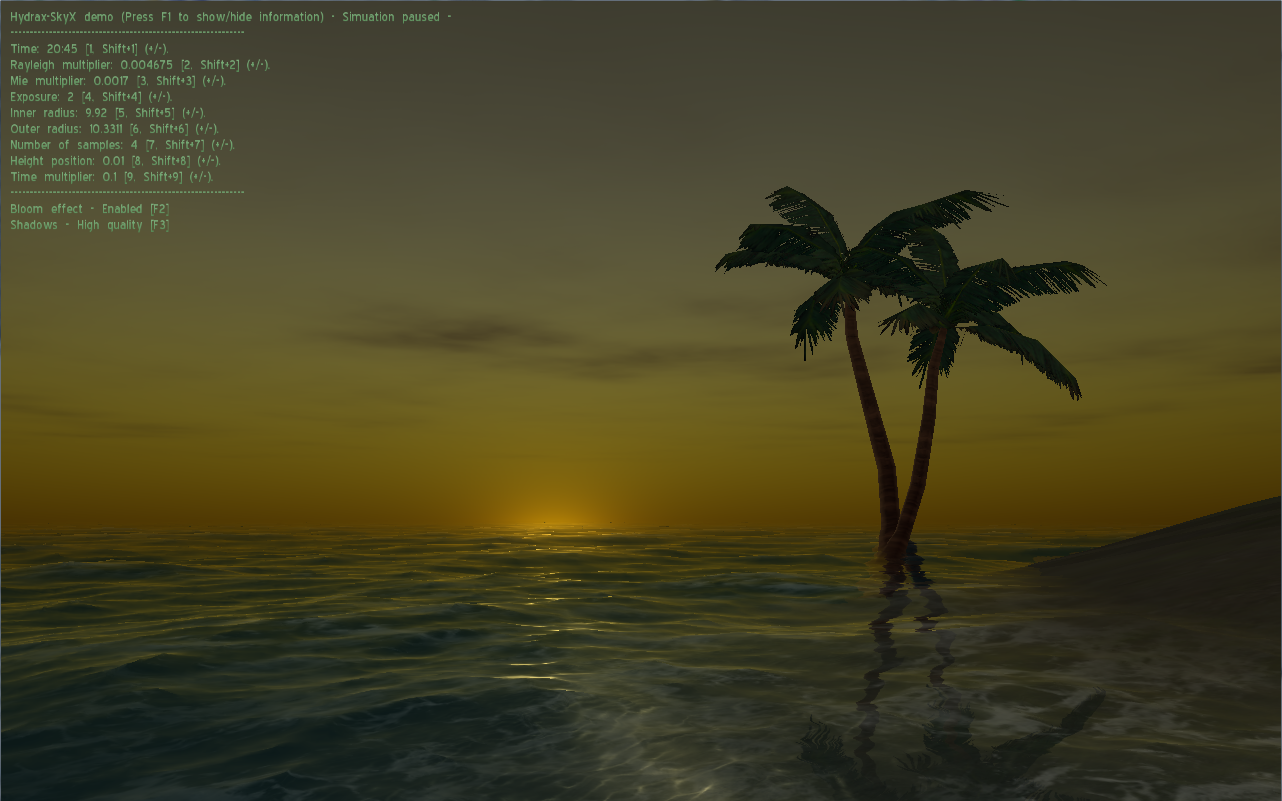
\includegraphics[scale=0.15]{hydrax} 
\end{figure}
\end{frame}

\begin{frame}{GUI}
\begin{columns}
  \begin{column}{0.5\textwidth}
    \textbf{\underline{Blender}} (\textcolor{red}{-98-38-2500} líneas)
    
    \vspace{0.4cm}
    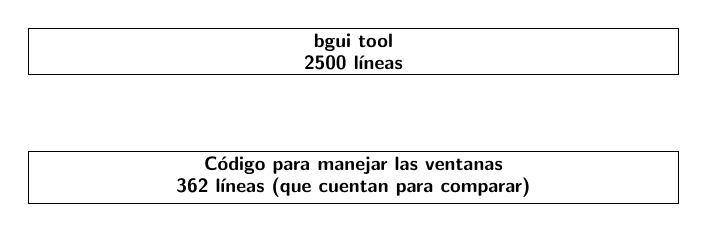
\begin{tikzpicture}[scale=0.8]
    	\node [whitebox] (bgui) at ($(-5,\vertspacing*1)$) {
    		\nodelabel{bgui tool}{\textit{2500 líneas}}
    	};
    	\node [whitebox] (Ventanas) at ($(-5,\vertspacing*3)$) {
    		\nodelabel{Código para manejar las ventanas}{\textit{362 líneas (que cuentan para comparar)}}
    	};
    \end{tikzpicture}
  \end{column}

  \begin{column}{0.5\textwidth}
    \textbf{\underline{OGRE}} (\textcolor{red}{-1054-379-159-11877-8220} líneas)
    
    \vspace{0.4cm}
    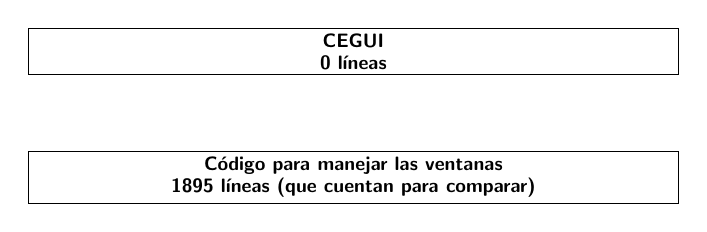
\begin{tikzpicture}[scale=0.8]
    	\node [whitebox] (CEGUI) at ($(-5,\vertspacing*1)$) {
    		\nodelabel{CEGUI}{\textit{0 líneas}}
    	};
    	\node [whitebox] (Ventanas) at ($(-5,\vertspacing*3)$) {
    		\nodelabel{Código para manejar las ventanas}{\textit{1895 líneas (que cuentan para comparar)}}
    	};
    \end{tikzpicture}
  \end{column}
\end{columns}
\end{frame}

\begin{frame}{Sonidos}
\begin{columns}
  \begin{column}{0.5\textwidth}
    \textbf{\underline{Blender}}
    
    (\textcolor{red}{-98-38-2500} líneas)
    
    \vspace{0.4cm}
    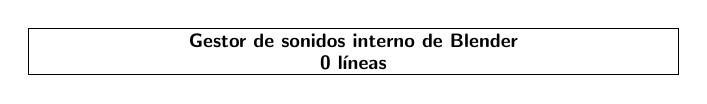
\begin{tikzpicture}[scale=0.8]
    	\node [whitebox] (Gestor de sonidos interno de Blender) at ($(-5,\vertspacing*1)$) {
    		\nodelabel{Gestor de sonidos interno de Blender}{\textit{0 líneas}}
    	};
    \end{tikzpicture}
  \end{column}

  \begin{column}{0.5\textwidth}
    \textbf{\underline{OGRE}}
    
    (\textcolor{red}{-1054-379-159-11877-8220-1880} líneas)
    
    \vspace{0.4cm}
    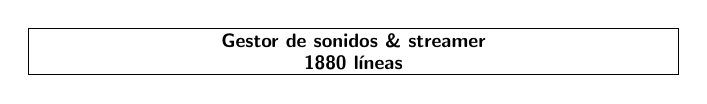
\begin{tikzpicture}[scale=0.8]
    	\node [whitebox] (Gestor de sonidos y streamer) at ($(-5,\vertspacing*1)$) {
    		\nodelabel{Gestor de sonidos \& streamer}{\textit{1880 líneas}}
    	};
    \end{tikzpicture}
  \end{column}
\end{columns}
\end{frame}

\begin{frame}{Entidades}
\begin{columns}
  \begin{column}{0.5\textwidth}
    \textbf{\underline{Blender}}
    
    (\textcolor{red}{-98-38-2500-2206-388} líneas)
    
    \vspace{0.4cm}
    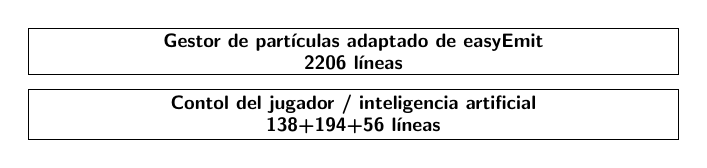
\begin{tikzpicture}[scale=0.8]
    	\node [whitebox] (easyEmit) at ($(-5,\vertspacing*1)$) {
    		\nodelabel{Gestor de partículas adaptado de easyEmit}{\textit{2206 líneas}}
    	};
    	\node [whitebox] (AI) at ($(-5,\vertspacing*2)$) {
    		\nodelabel{Contol del jugador / inteligencia artificial}{\textit{138+194+56 líneas}}
    	};
    \end{tikzpicture}
  \end{column}

  \begin{column}{0.5\textwidth}
    \textbf{\underline{OGRE}}
    
    (\textcolor{red}{-1054-379-159-11877-8220-1880-592} líneas)
    
    \vspace{0.4cm}
    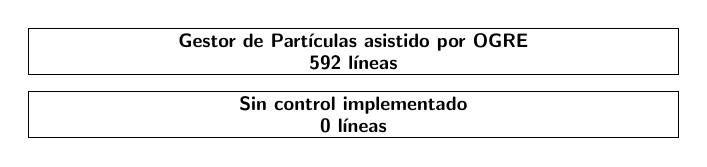
\begin{tikzpicture}[scale=0.8]
    	\node [whitebox] (particulas) at ($(-5,\vertspacing*1)$) {
    		\nodelabel{Gestor de Partículas asistido por OGRE}{\textit{592 líneas}}
    	};
    	\node [whitebox] (particulas) at ($(-5,\vertspacing*2)$) {
    		\nodelabel{Sin control implementado}{\textit{0 líneas}}
    	};
    \end{tikzpicture}
  \end{column}
\end{columns}
\end{frame}


\section{Conclusiones} 

\subsection{Resultado del experimento}
\begin{frame}{Resultado}
\begin{columns}
  \begin{column}{0.5\textwidth}
    \textbf{\underline{Blender}}
    
    \textbf{2745 líneas de código ``comparables''}

	\begin{figure}
		
\includegraphics[scale=0.15]{python_logo} 
	\end{figure}
  \end{column}

  \begin{column}{0.5\textwidth}
    \textbf{\underline{OGRE}}
    
    \textbf{15050 líneas de código ``comparables''}

	\begin{figure}
		
\includegraphics[scale=0.8]{C_plus_plus} 
	\end{figure}
  \end{column}
\end{columns}

\vspace{0.5cm}
Según la estimación (en la que he tratado de restringir al máximo los
efectos al cambio de lenguaje de programación) el código en C++ parece
requerir 5.5 líneas más de código que una implementación en Python.

\vspace{0.5cm}
La medida queda fuera del valor que obtuvimos muestreando
algunos algoritmos de ordenación ($2.7 \pm 1.6$).

\end{frame}

\subsection{Conclusiones}
\begin{frame}{Conclusiones}
\begin{itemize}
	\item Existe una gran cantidad de información y comparaciones fiables sobre la
	velocidad de códigos implementados en ambos lenguajes. \pause
	\item Existen estimaciones del número de errores que se cometen en cada
	lenguaje por línea de código escrita (0.69 vs. 0.005 bugs per KLOC). \pause
	\item No parecen existir estudios serios acerca de la diferencia de esfuerzo
	en el desarrollo dependiendo del lenguaje empleado.
	Por ejemplo, si en \CC $\,$ se requiren 10 líneas más de código que en Python
	para llevar a cabo la misma tarea, el índice de errores estará artificialmente
	incrementado un orden de magnitud. \pause
	\item Se ha tratado de estimar la influencia del lenguaje de programación
	en una aplicación compleja, usando como indicador el número de líneas
	de código. Para ello se ha tratado de eliminar todo elemento ``no comparable''.
	\pause
	\item Ambas aplicaciones son demasiado diferentes, así que el resultado no
	debe considerarse una buena medida. \pause
	\item Tal y como se podía esperar en \CC $\,$ se ha obtenido un incremento
	significativo de las líneas de código necesarias. \pause
	\item Tampoco se ha abordado la dependencia con el ámbito de aplicación.
\end{itemize}
\end{frame}

\subsection{Demostración}
\begin{frame}{Demostración}
\begin{center}
{\Huge Demo}
\end{center}
\end{frame}


\section{Demostración}
\begin{frame}{Demostración}
\begin{columns}
  \begin{column}{0.7\textwidth}
    \begin{center}
    {\Huge Demo}
    \end{center}
  \end{column}
  \begin{column}{0.3\textwidth}
    \begin{figure}
      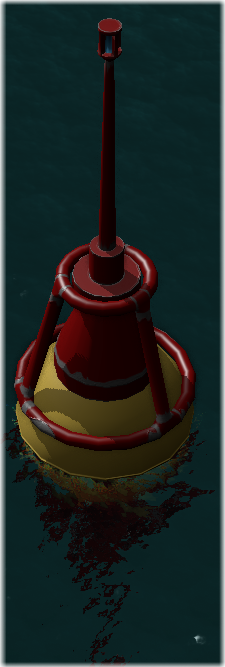
\includegraphics[scale=0.3]{demo} 
    \end{figure}
  \end{column}
\end{columns}
\end{frame}

\subsection{Física}

\begin{frame}{Creando la física}
Partimos de:
\begin{enumerate}
	\item Un objeto poco detallado para manejar la física.
	\item Dos objetos detallados sin propiedades físicas. Estos objetos tan sólo
	estarán ligados al objeto físico  que será invisible.
\end{enumerate}

Acciones a tomar:
\begin{enumerate}
	\item Retiramos la física a los dos objetos ``visuales''.
	\item Establecemos el controlador físico como dinámico:
	\begin{enumerate}
		\item $m = 4.6 \mathrm{ton}$
		\item $r = 1.3 \mathrm{m}$
		\item $r_{factor} = 1$
	\end{enumerate}
	También eliminamos todos los efectos disipativos.
\end{enumerate}

\end{frame}

\begin{frame}{Física implementada ``out of the box''}
El objeto ahora tiene la física implementada ``de serie'', y por tanto si
empezamos la simulación el objeto caerá irremediablemente.

Queremos por tanto implementar los efectos del agua.
\end{frame}

\subsection{Hidrodinámica}

\begin{frame}{Flotabilidad (hidrostática)}

\begin{center}
$\Delta = \rho \nabla$
\end{center}

$\Delta = $ Desplazamiento (peso del objeto)

$\rho = $ Densidad del agua

$\nabla = $ Volumen de agua desplazada

\begin{figure}
  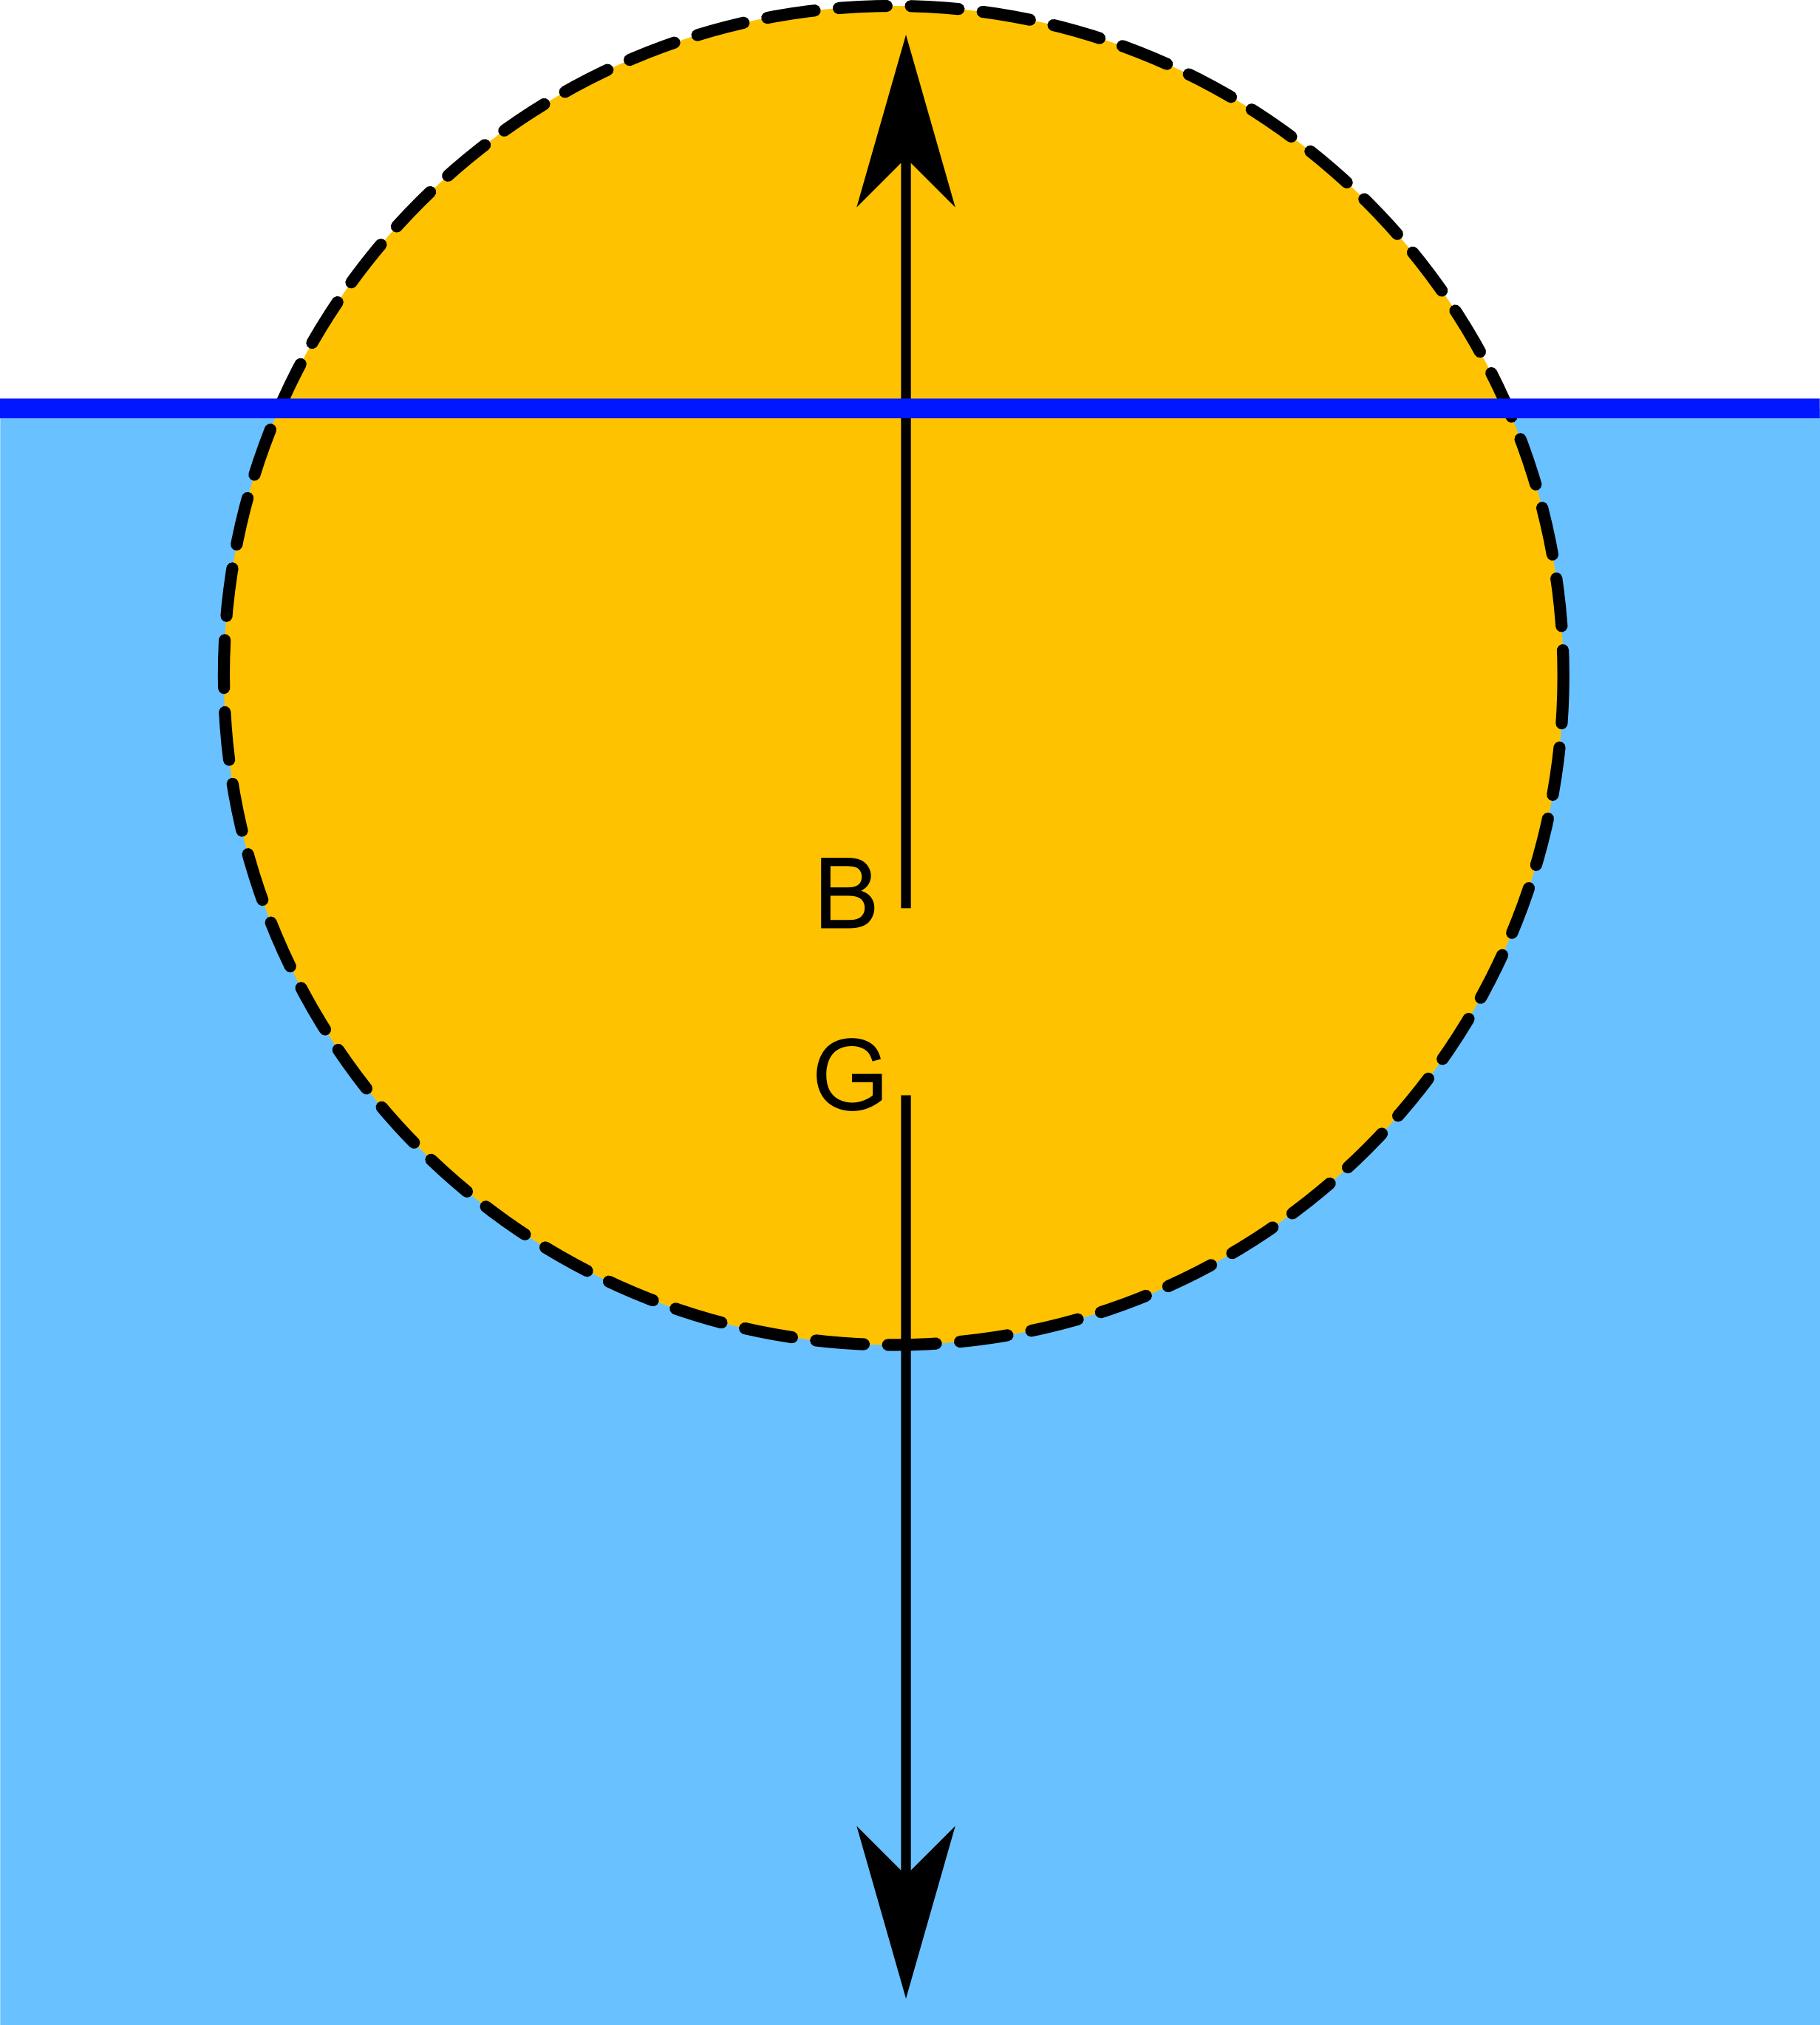
\includegraphics[scale=0.15]{archimedes} 
\end{figure}

\pause

\begin{center}
$\nabla = \frac{\pi}{3} \left( R - z \right)^2 \left( 2 R + z \right)$
\end{center}

$R = $ Radio de la esfera

$z = $ Altura del centro de la esfera con respecto de la superficie libre

\end{frame}

\begin{frame}{Flotabilidad (hidrodinámica)}

\begin{center}
$\frac{\partial^2 z}{\partial t^2} = \vert \mathbf{g} \vert \left( \Delta - \rho \nabla \right)
= f(z^3)
$
\end{center}

Movimiento no amortiguado, es decir, el objeto nunca llegará a estar en
equilibirio.
%
Lo solucionamos añadiendo un término amortiguador:

\begin{center}
$\frac{\partial^2 z}{\partial t^2} = \vert \mathbf{g} \vert \left( \Delta - \rho \nabla \right)
- K \Delta^{2/3} \left(\frac{\partial z}{\partial t}\right)^3$
\end{center}

Podemos usar el mismo término amortiguador para todos los movimientos en $x$,
$y$ y $z$.

\end{frame}

\begin{frame}{Estabilidad}

Excitación del mar del tipo:

\begin{center}
$M = A \cdot \cos\left( \omega t \right)$
\end{center}

Estabilidad regida por el parámetro $GM$:

\begin{figure}
  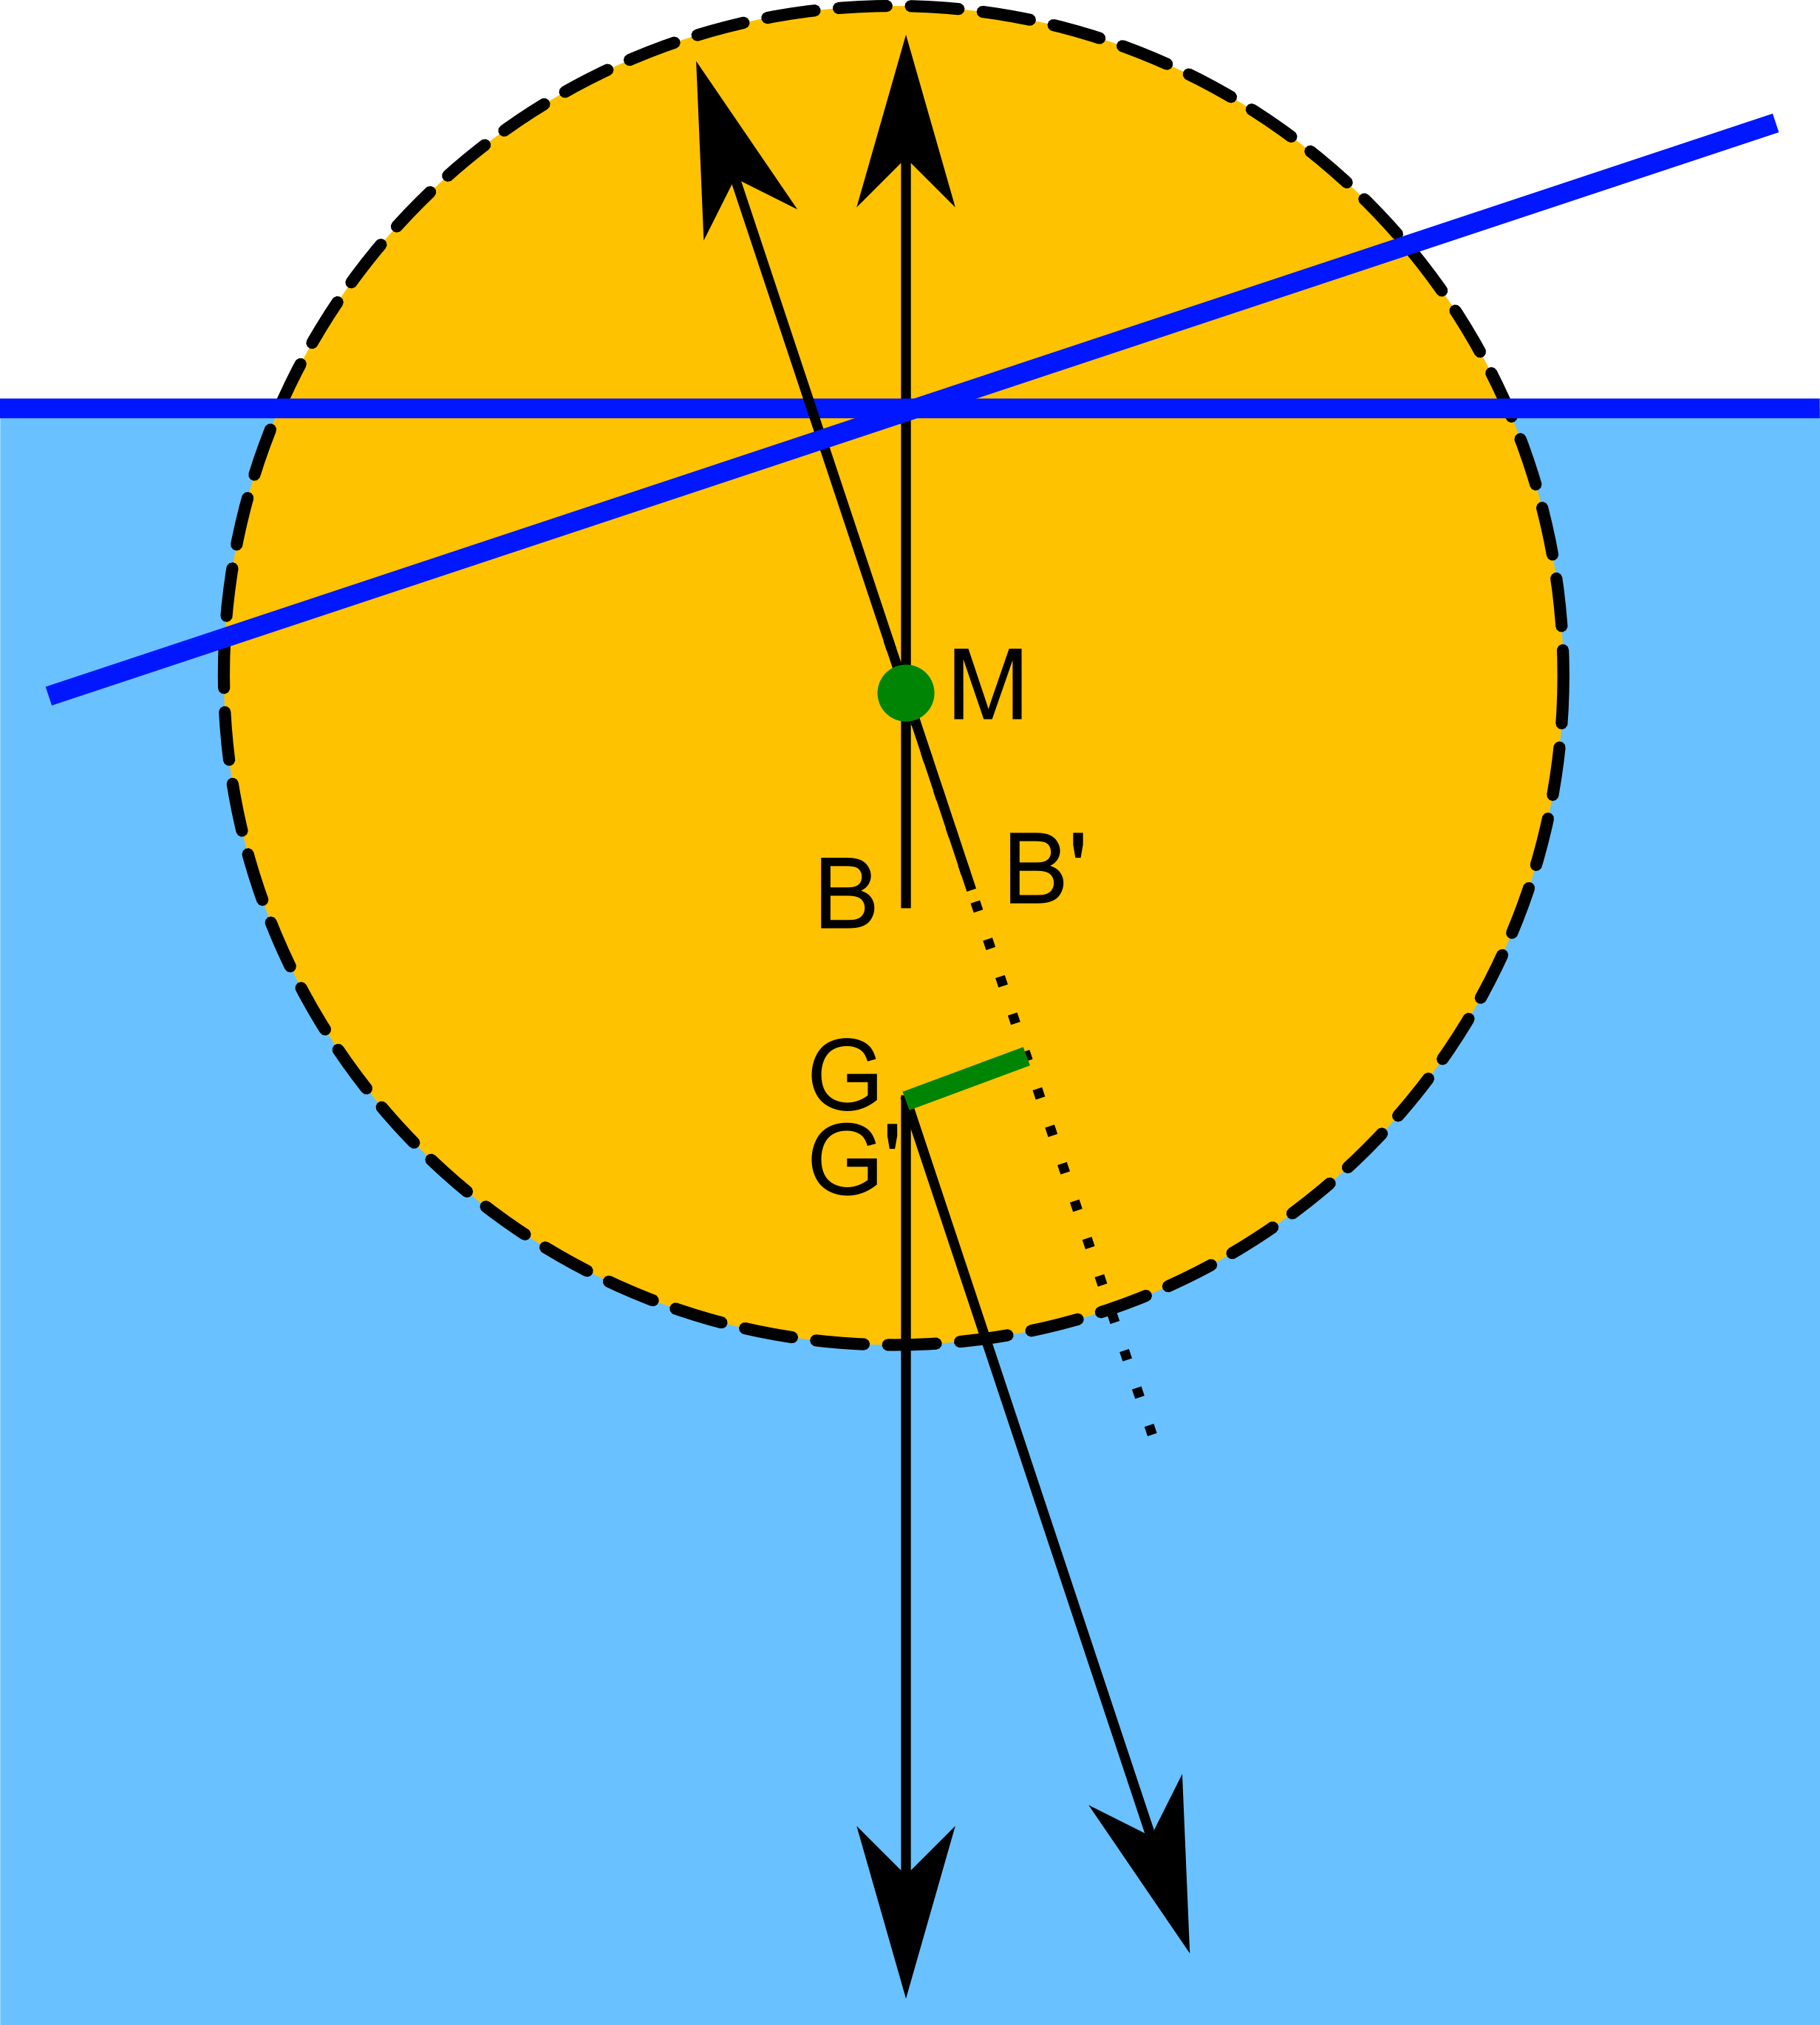
\includegraphics[scale=0.15]{stability} 
  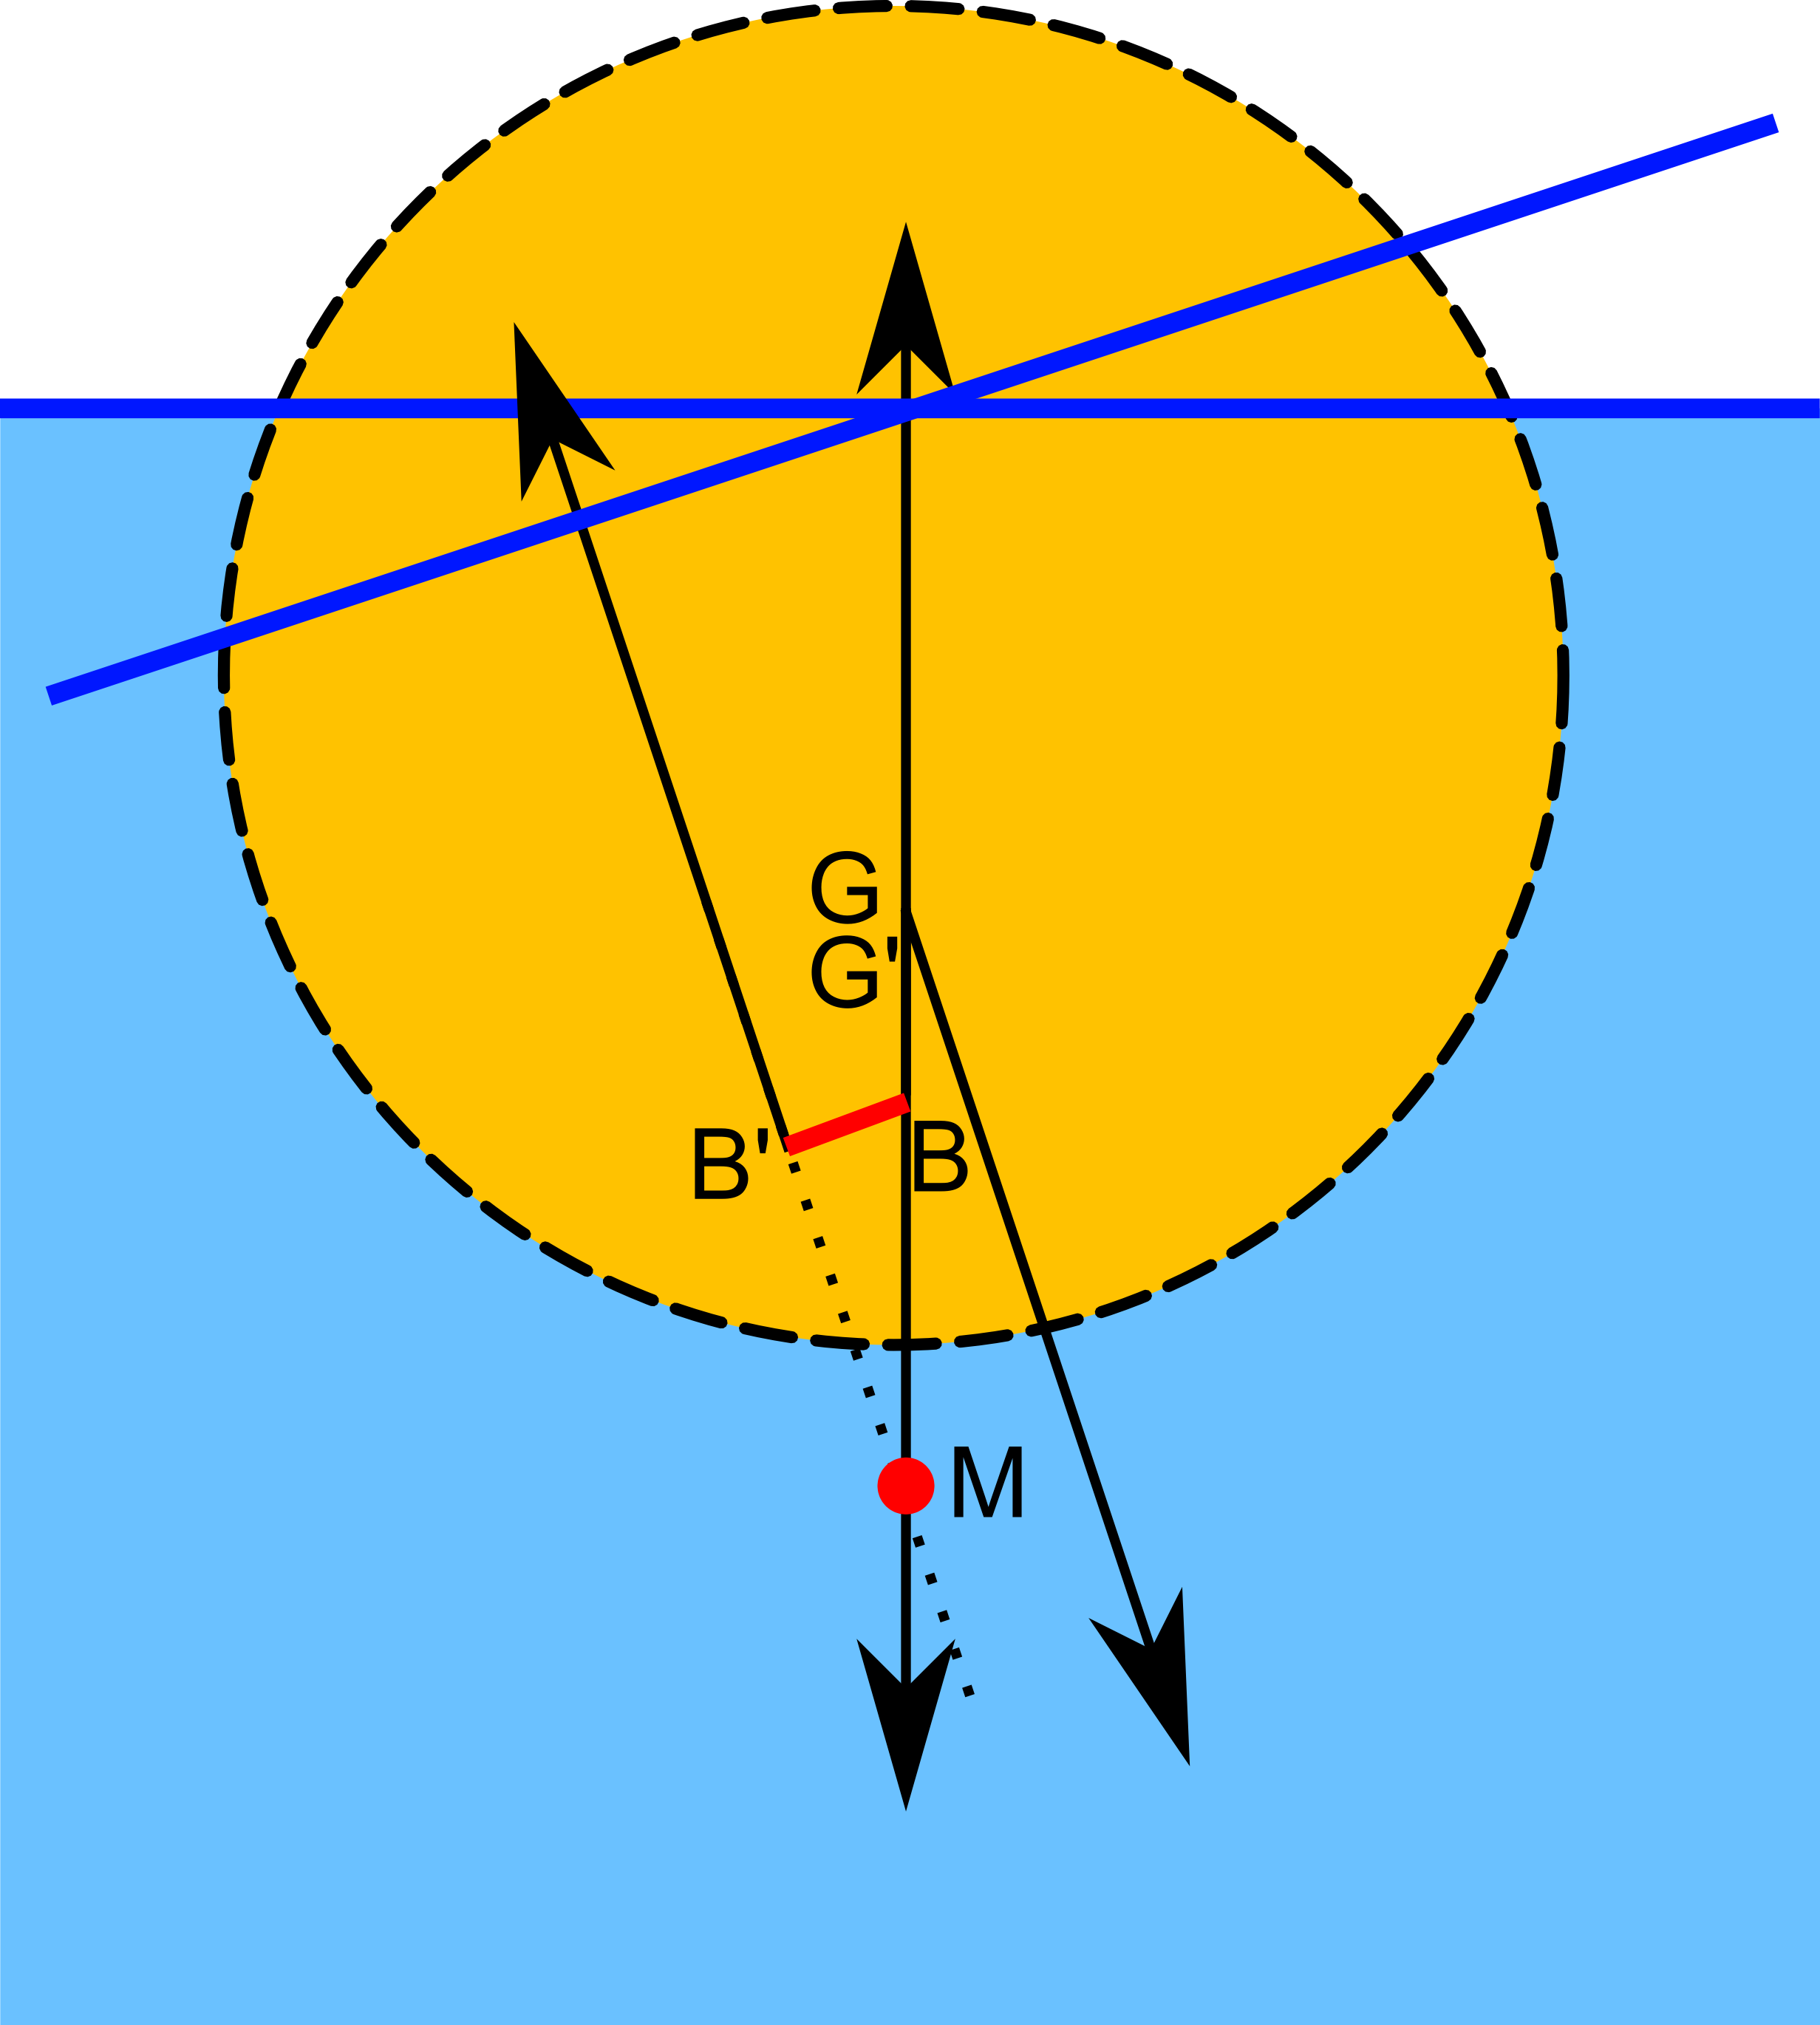
\includegraphics[scale=0.15]{stability_bad} 
\end{figure}

\pause

\begin{center}
$M = \vert \mathbf{g} \vert \Delta GM \sin\left( \theta \right)$
\end{center}

\pause

$\vert \left. \mathbf{u_x} \right\vert_{local}
\cdot
\vert \left. \mathbf{u_x} \right\vert_{global} = \cos\left( \theta \right)
\longrightarrow
\vert \left. \mathbf{u_x} \right\vert_{local}
\cdot
\vert \left. \mathbf{u_z} \right\vert_{global} = \sin\left( \theta \right)$

En este caso también añadimos un término viscoso.

\end{frame}

\subsection{Importando el nuevo objeto}

\begin{frame}{Preparación de la escena}

\begin{enumerate}
	\item Nos aseguramos de que todas las luces y cámaras (si las hubiera) se
	encuentran en capas inactivas.
	\item Colocamos todos los objetos útiles en una capa inactiva. De no hacerlo
	al cargar la ``librería'' el objeto se añadirá automáticamente a la escena,
	y no se podrán crear más instancias del mismo.
	\item Guardamos el archivo.
\end{enumerate}

\end{frame}

\begin{frame}[fragile]{Edición de la misión}

Cargamos la nueva ``librería'':
\begin{verbatim}
Manager.load_blender_file('AI/Bouy/Bouy.blend')
\end{verbatim}

Añadimos el objeto a la escena:
\begin{verbatim}
obj = scene.addObject('Bouy', origin)
\end{verbatim}

Y lo posicionamos:
\begin{verbatim}
obj.worldPosition = Vector((-190.0, 1900.0, 0.0))
\end{verbatim}

\begin{center}
{\Huge ¡Hecho!}
\end{center}

\end{frame}



\section{Conclusiones} 

\subsection{Conclusiones}
\begin{frame}{Conclusiones}
\begin{itemize}
	\item Blender ha puesto a disposición de los desarrolladores una herramienta
	rápida, flexible y potente. \pause
	\item Se trata de un motor gráfico joven (en comparación con otros software
	similares), y eso tiene algunas consecuencias negativas. \pause
	\item Aunque dicho motor tiene una buena integración con las herramientas de
	Blender, aún no se encuentra completamente integrado (por ejemplo no se pueden
	manipular las mallas desde el motor gráfico).
	\item Al estar amparada por un proyecto como Blender se puede esperar un buen
	soporte. \pause
	\item Durante ésta presentación hemos creado una entidad básica, mostrando lo
	sencillo que resulta. \pause
	\item Se ha mostrado como se puede modificar su comportamiento de forma
	sencilla mediante Python. \pause
\end{itemize}
\end{frame}

\begin{frame}{Fin}
\begin{center}
{\Huge ¡Muchas gracias!}

{\Huge ¿Preguntas?}
\end{center}
\end{frame}


\end{document}